\section{Ejercicio 3: Si esto no es el tesoro, el tesoro dónde está}
    % 1. Describir detalladamente el problema a resolver dando ejemplos del mismo y sus soluciones.
    \subsection{Descripción del problema}

		\begin{figure}[ht]
			\begin{center}
				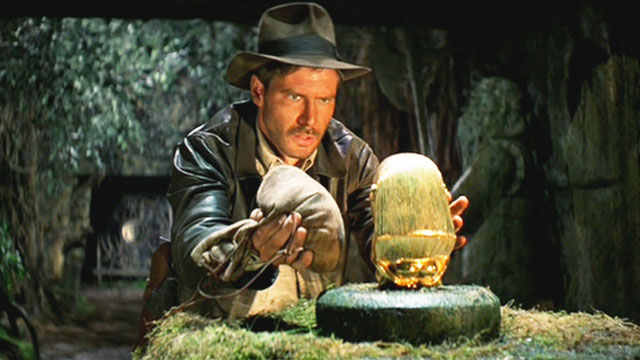
\includegraphics[width=0.4\columnwidth]{imagenes/tesoros.jpg}
				\caption{Fortuna y gloria muñeca, fortuna y gloria}
			\end{center}
		\end{figure}

        Una vez equilibrada la balanza, las paredes vuelven a su lugar. Con la llave obtenida logran abrir la puerta que estaba trabada. \par
		Al iluminar la habitación se encuentran con una sala de N tesoros. \par
		Por cada tipo de tesoro i, hay $C_{i}$ cantidades, con un valor $V_{i}$ y un peso $P_{i}$. Si bien el objetivo principal de la expedición era otro, nunca viene mal armarse de algún recuerdo. 
		Tienen M mochilas disponibles para llevarse los tesoros y cada una tiene una capacidad máxima de peso $K_{j}$ que puede llevar. \par
		El objetivo es llevarse el mayor valor posible de tesoros. Para esto, se debe devolver como resultado el valor total de tesoros guardados y además, por cada mochila, la cantidad de tesoros llevados y de qué tipo son.

        Por ejemplo, para la siguiente entrada:
        
        \begin{verbatim}
        M = 2
        K = { 1, 3 }
        
        N = 3 
        C = { 1, 2, 3 }
        V = { 2, 4, 10 }
        P = { 1, 2, 5 }
        \end{verbatim}

        Una posible salida válida sería:

        \begin{verbatim}
        S = 6
        M1 = { 1, 1 } 
        M2 = { 1, 2 }
        \end{verbatim}

        Es decir, para el caso en el que tenemos dos mochilas con capacidades 1 y 3, y nos encontramos con tres tesoros, el primero de peso 1 y valor 2, el segundo de peso 2 y valor 4, y el tercero de peso 5 y valor 10... \par Nos llevaremos en la primer mochila el primer tesoro y en la segunda el segundo tesoro. El tercer tesoro ya no nos entra.

    % 2. Explicar de forma clara, sencilla, estructurada y concisa, las ideas desarrolladas para la resolución del problema. Utilizar pseudocódigo y lenguaje coloquial (no código fuente). Justificar por qué el procedimiento resuelve efectivamente el problema.
    \subsection{Solución propuesta}
    Para solucionar el problema planteado se usó la técnica algorítmica de \emph{Programación dinámica}. \par

    La idea es separar el problema principal en subproblemas. En este caso, el subproblema es, en base a la capacidad restante de cada mochila y, al valor y peso de cada tesoro, en qué mochila conviene meter cada uno (incluyendo la opción de no meterlo en ninguna). Más formalmente el subproblema es: si ya resolvimos el beneficio máximo para los tesoros $T_{j}$, $j < i$, cómo se calcula el beneficio máximo teniendo en cuenta al $T_{i}$. Entonces la idea es la siguiente: si tenemos un solo tesoro (caso base) el máximo beneficio que se puede obtener es el valor del tesoro en caso de que entre en alguna mochila. Para el tesoro siguiente (recursión) el máximo beneficio que se puede obtener es el máximo entre: el valor del tesoro actual más el valor máximo que se podía llevar con el tesoro anterior con el peso restante de la mochila 1 al colocar este tesoro si entra, a esto lo llamaremos \textbf{ValorMochila1}, el mismo valor pero para la mochila 2 o \textbf{ValorMochila2}, el mismo valor pero para la mochila 3 o \textbf{ValorMochila3} , y así sucesivamente para las n mochilas y el valor que se obtiene si no se coloca, que sería el valor que se puede obtener para el tesoro anterior. Es decir la idea intuitiva es que en cada paso se compara el benficio de poner el tesoro en algunas de las mochilas con el beneficio de no ponerlo, en base al beneficio anterior. Podría verse como que se van comparando de a pares el beneficio de un tesoro y otro y nos quedamos con el mejor, siempre viendo todas las posilibidades de ponerlo en todas las mochilas, y despues de quedarse con la mejor opcion, se repite el procedimiento pero para el beneficio máximo calculado entre esos dos tesoros y uno que sigue. Se puede observar que el orden en el cual se recorren los tesoros no es importante. La solución que se obtiene luego de comparar con el último tesoro es óptima ya que en cada paso se está obteniendo el mayor beneficio,comparando todas las posibilidades. Se propone una función de recursión, la cual está definida en el rango 1..n, siendo n la cantidad de tesoros total y $\digamma(i)$ indicando el beneficio máximo que se puede obtener considerando los primeros i tesoros: \par

    $\digamma(1)$ = valor $v$ del primer tesoro si éste entra en alguna de las mochilas

    $\digamma(i)$ = max(valorMochila1,valorMochila2,valorMochila3, $\digamma(i-1)$)

    Lo que falta aclarar en esta función es que para cada tesoro se debe calcular el beneficio máximo que se puede obtener para cada peso posible de cada mochila, es decir se calculan los beneficios máximos para todos los posibles pesos de una mochila, desde uno hasta el peso P de la mochila, para que sea posible conocer cuál es el beneficio total que se puede obtener con el próximo tesoro, ya que se necesitaba para eso el beneficio que se puede obtener con el peso restante al poner un tesoro. 

    Por lo tanto, el algoritmo propuesto consta de una matriz para cada tesoro, de tamaño $\[\prod_{i=0}^{3}C_{i} + 1$, siendo $C_{i}$ las capacidades de las \textbf{M} mochilas, donde $M \leq 3$. Y además una matriz nula de igual dimensión que servirá para el caso en donde no hayan tesoros. \par

    El algoritmo funciona de la siguiente manera:
    1) Se crea una matriz de $\[\prod_{i=0}^{M}C_{i} + 1$ para cada tesoro, y una extra inicial con los valores de todas las posiciones inicializados en 0.

    \begin{codesnippet}
    \begin{verbatim}
    for i = 1 .. cantTesoros + 1
        for j = 1 .. capacidadMochila1 + 1
            for k = 1 .. capacidadMochila2 + 1  
                for l = 1 .. capacidadMochila3 + 1  
                    matriz[i][j][k][l] <-- 0
                end
            end
        end
    end
    \end{verbatim}
    \end{codesnippet}


    2) En el caso donde $M < 3$, el programa se encarga de fijar las capacidades de las $3 - M$ mochilas en 0.
    Para cada posición (i, j, k) de la matriz del tesoro t, siendo i, j y k la capacidad \emph{restante} de las mochilas 1, 2 y 3, se pregunta si t entra en alguna de las tres mochilas.
    Si entra en la mochila 1, se obtiene valor(t) sumado al valor de la matriz del tesoro t-1 (recordar que el primer tesoro tiene una matriz predecesora con todos sus valores nulos) en la posición correspondiente según la capacidad restante de esa mochila (i - peso(t), j, k).
    Se repite este procedimiento para cada mochila. 
    Y además se obtiene el valor de la posición (i, j, k) de la matriz del tesoro t-1 para incluir el caso en el que no se mete el objeto en la mochila.
    Luego se obtiene el resultado mayor de cada suma, y se guarda en la matriz del tesoro t, en la posición (i, j, k)..

    \begin{codesnippet}
    \begin{verbatim}

    valorMochila1 = 0
    valorMochila2 = 0
    valorMochila3 = 0

    valorNingunaMochila = matriz[t-1][i][j][k]


    if (pesoTesoro <= i ||pesoTesoro <= j || pesoTesoro <= k)

        if pesoTesoro <= i then
            valorMochila1 <-- valor(t) + matriz[t-1][i - pesoTesoro][j][k]
        endif

        if pesoTesoro <= j then
            valorMochila2 <-- valor(t) + matriz[t-1][i][j - pesoTesoro][k]
        endif

        if pesoTesoro <= k then
            valorMochila3 <-- valor(t) + matriz[t-1][i][j][k - pesoTesoro]
        endif
    
        matriz[t][i][j][k] <-- max(valorMochila1, valorMochila2, valorMochila3, valor(t-1))
    else
        matriz[t][i][j][k] < -- valor(t-1)


    

    \end{verbatim}
    \end{codesnippet}

    Se repite este procedimiento para cada tesoro, hasta completar todas las posiciones de cada matriz.
    El último valor obtenido de la matriz del último tesoro, será el valor máximo que se puede acumular en las mochilas con los tesoros.

    3) Luego, empezando desde la matriz del último tesoro, desde la última posición (i, j, k), se pregunta si entra ese tesoro en alguna mochila. 
    Si no entra, se repite el procedimiento para el tesoro anterior.
    Si entra, se pregunta en cuáles de las mochilas entra ese tesoro. Para eso se guarda la capacidad disponible de cada mochila (inicialmente con su capacidad total) y se pregunta si el tesoro tiene peso menor o igual a cada capacidad.
    En caso de que entre en más de una mochila, se compara el valor resultante de ponerlo en cada una. Por ejemplo, para la mochila 1, se obtiene el valor de la posición (i - peso(t), j, k) de la matriz del tesoro t-1.
    Una vez obtenido en qué mochila es conveniente poner a ese tesoro, se almacena en cada vector de salida (hay uno por mochila) los tipos de tesoro que guardo en cada mochila. Se incrementa el contador de tesoros de esa mochila, y luego el indice pasa a ser aquella posición donde estaba el valor máximo. Por ejemplo, si la mejor opción es guardar ese tesoro en la mochila 1, (i, j, k) pasa a ser (i - peso(t), j, k), t pasa a ser t-1, y se le resta peso(t) a la capacidad restante de esa mochila.

    \begin{codesnippet}
    \begin{verbatim}

    entraEnAlgunaMochila <-- matriz[t+1][i][j][k] != matriz[t][i][j][k]

    if entraEnAlgunaMochila then
    	valorAnterior1 <-- 0
    	valorAnterior2 <-- 0
        valorAnterior3 <-- 0
	    entraEnMochila1 <-- (pesoTesoro <= i);
		entraEnMochila2 <-- (pesoTesoro <= j);
        entraEnMochila3 <-- (pesoTesoro <= k);

		if entraEnMochila1 then
			valorAnterior1 <-- matriz[t][i - pesoTesoro][j][k]
		endif
		if entraEnMochila2 then
			valorAnterior2 <-- matriz[t][i][j - pesoTesoro][k]
		endif
        if entraEnMochila2 then
            valorAnterior3 <-- matriz[t][i][j][k - pesoTesoro]

		if entraEnMochila1 && valorAnterior1 >= valorAnterior2  && valorAnterior1 >= valorAnterior3
        then
			add(mochila1, tipo(t))
			cantTesorosMochila1++
			i -= peso(t)
		else if entraEnMochila2 && valorAnterior2 >= valorAnterior3 
			add(mochila2, tipo(t))
			cantTesorosMochila2++
			j -= peso(t)
        else
            add(mochila3, tipo(t))
            cantTesorosMochila3++
            k -= peso(t)
		endif

	endif

    \end{verbatim}
    \end{codesnippet}

    Se repite este procedimiento para cada tesoro.

    4) Una vez finalizados los primeros tres pasos, se copia en una tupla el valor obtenido entre todos los tesoros guardados en las mochilas, y un vector mochilas que contiene un vector por mochila. Cada uno de estos vectores guarda la cantidad de tesoros y los tipos de tesoro que hay en esa mochila.


   
    \subsection{Complejidad teórica}
        Para analizar la complejidad teórica, vamos a hacer referencia a la \textbf{implementación} del algoritmo.
        Para esto, el mismo, puede ser dividido en varias etapas independientes, donde al final, sus complejidades serán sumadas, dando así la complejidad teórica final. Las etapas son, 

        \begin{itemize}
            \item En primer lugar, se inicializan ciertas variables necesarias para el algoritmo en $\ord(1)$, además de inicializar la variable \emph{capacidades}, en la cual se insertan las capacidades de las distintas mochilas. Siendo M la cantidad de mochilas, y $\ord(1)$ la operación de \emph{incersión} en un vector, esto da un total de $\ord(M)$ la inicialización de variables.
            \item Además de las variables, se inicializa un vector de matrices denominado \textbf{cuboMagico}. Las mismas serán usadas para almacenar las ganancias acumuladas de llevar un tesoro o no. Para esto, sea N los tipos de tesoros y $C_{i}$ la cantidad del tesoro de tipo i, se redimensionará el vector de matrices cuboMagico por cada uno de los tesoros además de una matriz nula. Es decir en 
            $\ord(\sum_{i = 0}^{N-1} C_{i} + 1)$ inicializa el vector de matrices.
            \item Luego sea T, la cantidad de tesoros total más la matríz nula, es decir
            $T = \sum_{i = 0}^{N-1} C_{i} + 1$
            A cada matríz se la redimensionará con la capacidad de las M mochilas. O sea para cada tesoro, se inicializa una matriz cuyas dimensiones son $ \prod_{i = 0}^{M-1} K_{i}$. Esta inicialización tiene una cota asintótica de $\ord((\prod_{i = 0}^{M-1} K_{i}})*T)$.
            \item Luego recorro cada una de las matrices, para sumar el valor acumulado por cada posición de cada matriz. Esto es, recorrer todas las matrices una vez cada una tiene un costo de complejidad de $\ord((\prod_{i = 0}^{M-1} K_{i}})*T)$.

            \item Finalmente debo recorrer desde la última matriz hasta la primera. Cada vez que el algoritmo determine que un tesoro es óptimo para llevar en una mochila, el tesoro será ingresado al vector de cada mochila. La inserción de un elemento a un vector es $\ord(1)$.Pero recorrer todas las matrices vuelve a tener una complejidad de $\ord((\prod_{i = 0}^{M-1} K_{i}})*T)$.


        \end{itemize}


        Por lo visto anteriormente, el algoritmo tiene complejidad temporal de\par

        \[
            \ord(M) + \ord(T) + \ord((\prod_{i = 0}^{M-1} K_{i})*T) =
        \]
        \[
            \ord(M + (\prod_{i = 0}^{M-1} K_{i})*T) =
        \]
        \[
            \ord((\prod_{i = 0}^{M-1} K_{i})*T) =
        \]
        \[
            \ord((\prod_{i = 0}^{M-1} K_{i})*(\sum_{i = 0}^{N-1} C_{i} + 1)) =
        \]
        Luego, la complejidad final de nuestro algoritmo es\par
        \[
            \ord((\prod_{i = 0}^{M-1} K_{i})*(\sum_{i = 0}^{N-1} C_{i}))
        \]

        Dado que nuestra cota máxima por enunciado era $\ord((\sum_{i = 0}^{M-1} K_{i})^{M}*(\sum_{i = 0}^{N-1} C_{i}))$ resta demostrar que. \par
        \[
            \prod_{i = 0}^{M-1} K_{i} \leq (\sum_{i = 0}^{M-1} K_{i})^{M}
        \]
        Para esto, podemos desarrollar la productoria y la sumatoria como,\par
        \[
            \prod_{i = 0}^{M-1} K_{i} = K_{0} * K_{1} * \dots * K_{M-1}
        \]
        \[
            (\sum_{i = 0}^{M-1} K_{i})^{M} = (K_{0} + K_{1} + \dots + K_{M-1})^{M}
        \]
        Resta probar que, \par
        \[
            K_{0} * K_{1} * \dots * K_{M-1} \leq (K_{0} + K_{1} + \dots + K_{M-1})^{M}
        \]
        Sea $K_{j}$ la mayor capacidad de todas, entonces \par
        \[
            K_{0} * K_{1} * \dots * K_{M-1} \leq (K_{j})^{M}
        \]
        Luego por propiedad de polinomios, seguro $(K_{j})^{M}$ pertenece a algún coeficiente de elevar a la M\par
        \[
            (K_{0} + K_{1} + \dots + K_{M-1})^{M}
        \]
        Además todos los coeficientes $K_{i} \neq K_{j}$ son positivos. \par
        Por lo tanto se demostró que $K_{0} * K_{1} * \dots * K_{M-1}  \leq (K_{j})^{M} \leq  (K_{0} + K_{1} + \dots + K_{M-1})^{M}$ \par
        Es decir, $\prod_{i = 0}^{M-1} K_{i} \leq (\sum_{i = 0}^{M-1} K_{i})^{M}$. \par
        Luego la cota dada es correcta. \par
    

    % 4. Dar un código fuente claro que implemente la solución propuesta. Se deben incluir las partes relevantes del código como apéndice del informe impreso entregado.

    % 5. Realizar una experimentación computacional para medir la performance del programa implementado. Usar un conjunto de casos de test en función de los parámetros de entrada, con instancias aleatorias e instancias particulares (de peor/mejor caso en tiempo de ejecución, por ejemplo). Presentar en forma gráfica una comparación entre los tiempos medidos y la complejidad teórica calculada y extraer conclusiones.
    \subsection{Experimentación}

        Al igual que con los otros dos ejercicios, se realizaron pruebas experimentales para verificar que el tiempo de ejecución del algoritmo cumpliera con la cota asintótica de $(\ord((\prod_{i = 0}^{M-1} K_{i})*(\sum_{i = 0}^{N-1} C_{i}))$, teóricamente demostrada para el peor caso. Las pruebas que se realizaron consistieron de probar con distinta cantidad de tamaños para 1 a 3 mochilas, donde la cantidad de tesoros era igual a los tamaños de las mochilas. El objetivo era observar el tiempo que toma el algoritmo cambiando estos valores. Para cada tesoro, su peso y valor fue un número random entre 1 y el tamaño de la mochila, tomado utilizando random de la librería estandar y con una distribución uniforme.
        El resultado de este experimento puede visualizarse en este gráfico:


      \begin{figure}[H]
      \begin{center}
        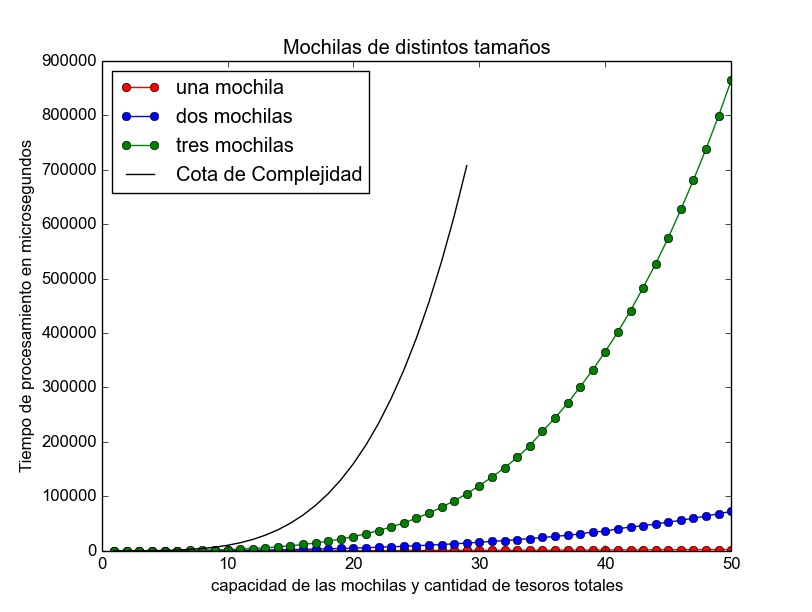
\includegraphics[width=0.7\columnwidth]{imagenes/ej3Nuevo.jpeg}
        \caption{}
      \end{center}
      \end{figure}

        Luego en base a los resultados, se puede observar que dentro de las variables es la cantidad de mochilas una de las que influye fuertemente en el tiempo de ejecución. Esto se debe pues, como fue explicado en la \textbf{solución propuesta}, a que las dimensiones de las matrices a recorrer, son del tamaño de la capacidad de las mochilas. Por esto a mayor cantidad de mochilas y mayor capacidad, el tiempo de ejecución es mayor. Por otro lado se puede obesrvar, que la complejidad teórica calculada es correcta según la experimentación.